
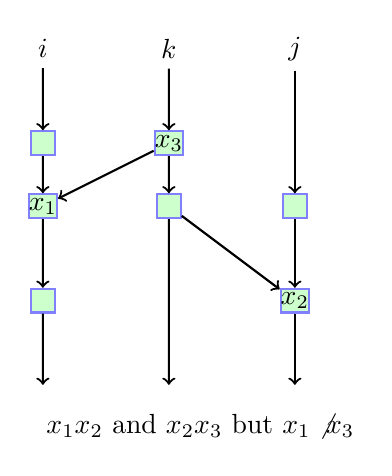
\begin{tikzpicture}[scale=0.4]
	\node 	(e0)		at	(-7,10) 	[rectangle, thick]{$i$};

	\node 	(e1)		at	(-7,7) 	[rectangle, thick, draw=blue!50,fill=green!20,inner sep=0pt,minimum size=.3cm]{$$};

	\node 	(e2)		at	(-7,5) 	[rectangle, thick, draw=blue!50,fill=green!20,inner sep=0pt,minimum size=.3cm]{$x_1$};

	\node 	(e3)		at	(-7,2) 	[rectangle, thick, draw=blue!50,fill=green!20,inner sep=0pt,minimum size=.3cm]{$$};

	\node 	(e4)		at	(-7,-1) 	[rectangle, thick]{};


	\draw[->, thick]	(e0)	to	node[auto]{}	(e1);
	\draw[->, thick]	(e1)	to	node[auto]{}	(e2);
	\draw[->, thick]	(e2)	to	node[auto]{}	(e3);
	\draw[->, thick]	(e3)	to	node[auto]{}	(e4);

	\node 	(f0)		at	(-3,10) 	[rectangle, thick]{$k$};

	\node 	(f1)		at	(-3,7) 	[rectangle, thick, draw=blue!50,fill=green!20,inner sep=0pt,minimum size=.3cm]{$x_3$};

	\node 	(f2)		at	(-3,5) 	[rectangle, thick, draw=blue!50,fill=green!20,inner sep=0pt,minimum size=.3cm]{$$};

%	\node 	(f3)		at	(-3,2) 	[rectangle, thick, draw=blue!50,fill=green!20,inner sep=0pt,minimum size=.3cm]{$$};

	\node 	(f3)		at	(-3,-1) 	[rectangle, thick]{};

	\draw[->, thick]	(f0)	to	node[auto]{}	(f1);
	\draw[->, thick]	(f1)	to	node[auto]{}	(f2);
	\draw[->, thick]	(f2)	to	node[auto]{}	(f3);
%	\draw[->, thick]	(f3)	to	node[auto]{}	(f4);


%	\node 	(e)		at (-4.5,-2) [rectangle, thick]{$\chi(e,j)=\down e\cup \up e$};
%	\draw[->, very thick]	(f1)	to	node[auto]{}	(e1);
%	\draw[->, very thick]	(e2)	to	node[auto]{}	(f2);
%	\draw[->, very thick]	(e3)	to	node[auto]{}	(f3);

%----------------------------------------------------------------------------------------

	\node 	(e0')		at	(1,10) 	[rectangle, thick]{$j$};

%	\node 	(e1')		at	(1,8) 	[rectangle, thick, draw=blue!50,fill=green!20,inner sep=0pt,minimum size=.3cm]{$$};

%	\node 	(e5')		at	(1,6.5) 	[rectangle, thick, draw=blue!50,fill=green!20,inner sep=0pt,minimum size=.3cm]{$$};

	\node 	(e1')		at	(1,5) 	[rectangle, thick, draw=blue!50,fill=green!20,inner sep=0pt,minimum size=.3cm]{$$};

%	\node 	(e6')		at	(1,3.5) 	[rectangle, thick, draw=blue!50,fill=green!20,inner sep=0pt,minimum size=.3cm]{$$};

	\node 	(e2')		at	(1,2) 	[rectangle, thick, draw=blue!50,fill=green!20,inner sep=0pt,minimum size=.3cm]{$x_2$};

	\node 	(e3')		at	(1,-1) 	[rectangle, thick]{};

	\draw[->, thick]	(e0')	to	node[auto]{}	(e1');
	\draw[->, thick]	(e1')	to	node[auto]{}	(e2');
	\draw[->, thick]	(e2')	to	node[auto]{}	(e3');
%	\draw[->, thick]	(e3')	to	node[auto]{}	(e4');



%----------------------------------------------------------------------------------------
	\draw[->, thick]	(f1)	to	node[auto]{}	(e2);
	\draw[->, thick]	(f2)	to	node[auto]{}	(e2');
%	\draw[->, thick]	(e3')	to	node[auto]{}	(e4');

%----------------------------------------------------------------------------------------

	\node 	(g)		at	(-2,-2) 	[rectangle, thick]{$\down x_1 \pres \down x_2 ~\mbox{and}~ \down x_2 \pres \down x_3 ~\mbox{but}~ \down x_1 \not \pres \down x_3$};
%
\end{tikzpicture}

%
%


